\chapter{Control de versiones y colaboración}

\section{Aplicación de Git con Conventional Commits}

\subsection{¿Qué son los Conventional Commits y por qué se usan?}
\emph{Conventional Commits} es un estándar para redactar mensajes de commit con una estructura fija: \texttt{tipo(alcance): descripción}. El \texttt{tipo} indica la naturaleza del cambio (nueva funcionalidad, corrección, documentación, etc.) y el \texttt{alcance}, opcional, precisa el módulo afectado (por ejemplo \texttt{backend}, \texttt{frontend} o \texttt{db}).

Adoptamos esta convención porque cada integrante trabajaba sobre una capa distinta del sistema, y el alcance indicado entre paréntesis permite identificar el componente afectado por cada cambio. Por ejemplo, el mensaje \texttt{feat(backend): agregar endpoints CRUD de notas} indica, sin necesidad de revisar el código, que se trata de una nueva funcionalidad del backend.

\subsection{Tipos principales}
\begin{itemize}
  \item \texttt{feat}: nueva funcionalidad.
  \item \texttt{fix}: corrección de errores.
  \item \texttt{docs}: cambios en documentación.
  \item \texttt{test}: cambios en pruebas.
  \item \texttt{chore}: tareas de mantenimiento.
  \item \texttt{ci}: cambios en integración continua.
  \item \texttt{refactor}: refactorización sin cambiar comportamiento.
\end{itemize}

\begin{notebox}
En el historial actual del proyecto se emplearon cinco de estos tipos: \textcolor{gitfeat}{\textbf{feat}} (nueva funcionalidad de DB, backend y frontend), \textcolor{gitchore}{\textbf{chore}} (configuración de Docker y del repositorio), \textcolor{gitdocs}{\textbf{docs}} (documentación), \textcolor{gitrefactor}{\textbf{refactor}} (reorganización de carpetas) y \texttt{test} (pruebas unitarias y automatización). Los tipos \texttt{fix} y \texttt{ci} aún no se han utilizado.
\end{notebox}

\subsection{Historial de commits}

\begin{figure}[H]
    \centering
    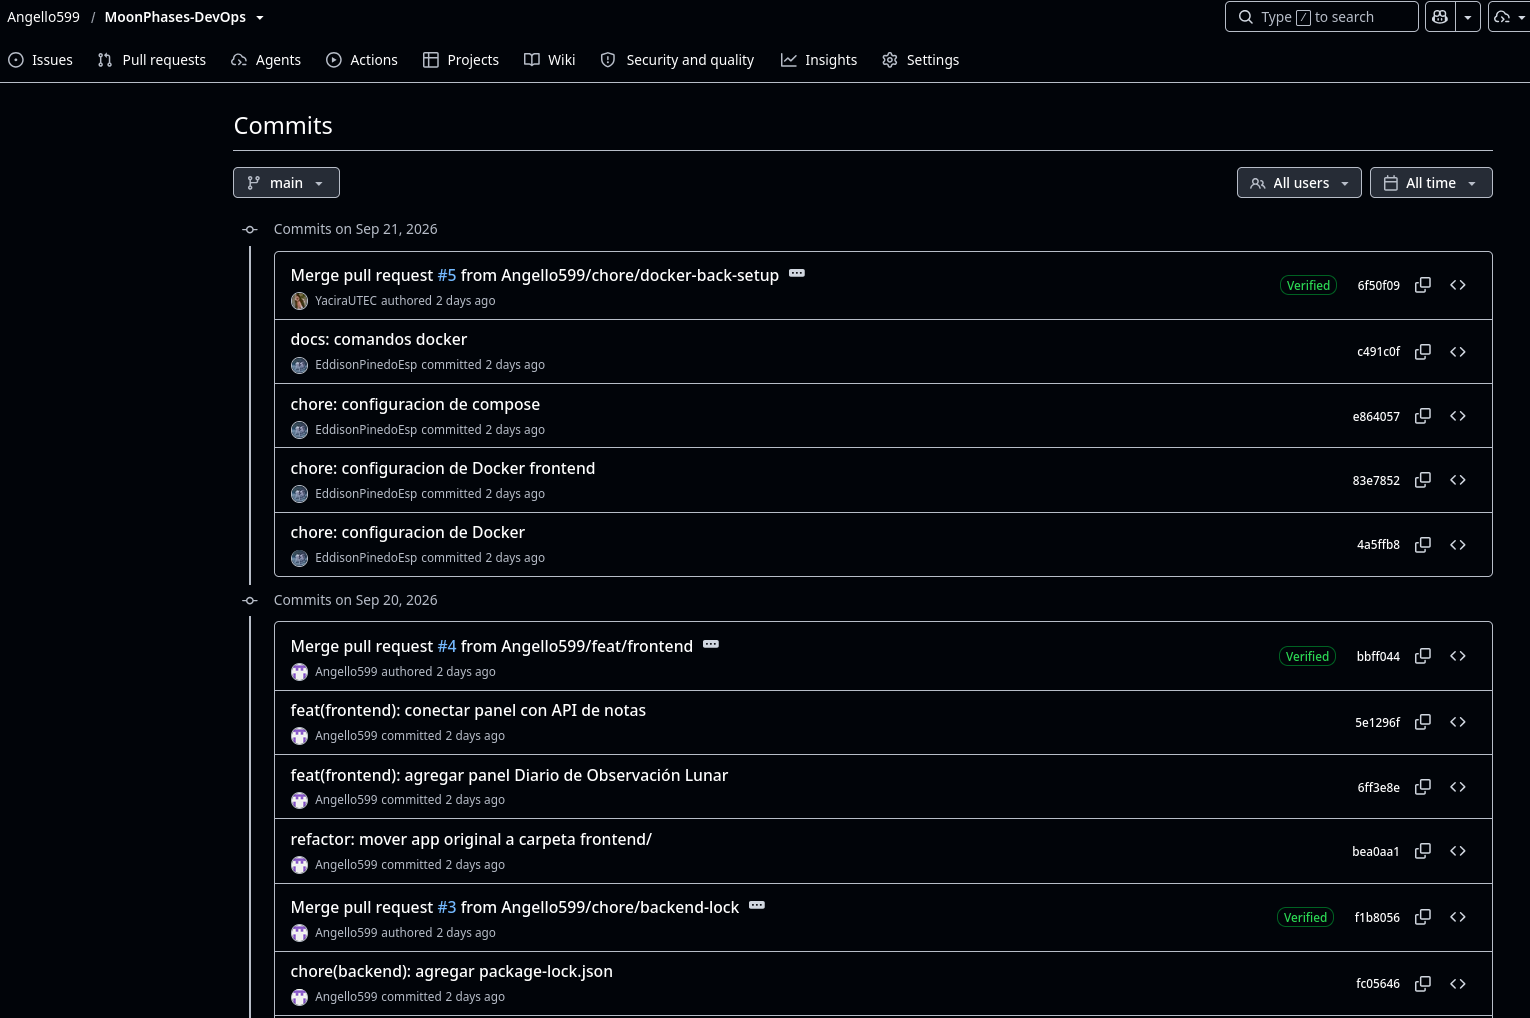
\includegraphics[width=0.92\textwidth]{content/imgs/commits.png}
    \caption{Historial de commits del repositorio \texttt{MoonPhases-DevOps} sobre la rama \texttt{main}, visualizado en GitHub.}
\end{figure}

El historial de \texttt{main} contiene 25 commits (17 commits de contenido y 8 commits de \emph{merge} de \emph{pull requests}). A continuación se analiza en detalle una muestra de 8 commits que recorre la evolución del proyecto desde la importación del código base hasta la incorporación de pruebas y su documentación.

\begin{center}
\begin{tabularx}{\textwidth}{@{}l l l >{\raggedright\arraybackslash}X@{}}
\toprule
\textbf{Hash} & \textbf{Tipo} & \textbf{Alcance} & \textbf{Mensaje y análisis} \\
\midrule

\texttt{e8c8428} &
\textcolor{gitchore}{\texttt{chore}} &
\textit{(repo)} &
\textbf{chore: importar código base de MoonPhases.}
Commit inicial que trae el proyecto original de NeaByteLab al repositorio del equipo, estableciendo el punto de partida sobre el que se construirán backend y base de datos. \\
\addlinespace

\texttt{0e24ea5} &
\textcolor{gitfeat}{\texttt{feat}} &
\texttt{db} &
\textbf{feat(db): agregar esquema de tabla moon\_notes.}
Define la tabla \texttt{moon\_notes} (fecha única, contenido, marcas de tiempo) en \texttt{backend/db/schema.sql}, la base de toda la persistencia de notas del diario lunar. \\
\addlinespace

\texttt{afeafb4} &
\textcolor{gitfeat}{\texttt{feat}} &
\texttt{backend} &
\textbf{feat(backend): agregar endpoints CRUD de notas.}
Implementa las rutas \texttt{GET/POST/DELETE} de \texttt{/api/notes} en Express, completando la API que el frontend consumirá más adelante. \\
\addlinespace

\texttt{bea0aa1} &
\textcolor{gitrefactor}{\texttt{refactor}} &
\textit{(repo)} &
\textbf{refactor: mover app original a carpeta frontend/.}
Reorganiza el repositorio monolítico en una estructura de módulos (\texttt{frontend/}, \texttt{backend/}), condición necesaria para poder dockerizar cada servicio de forma independiente. \\
\addlinespace

\texttt{6ff3e8e} &
\textcolor{gitfeat}{\texttt{feat}} &
\texttt{frontend} &
\textbf{feat(frontend): agregar panel Diario de Observación Lunar.}
Añade el componente \texttt{NotesPanel.ts}, la interfaz donde la persona usuaria escribe y consulta sus notas sobre la fase lunar. \\
\addlinespace

\texttt{c491c0f} &
\textcolor{gitdocs}{\texttt{docs}} &
\texttt{docker} &
\textbf{docs: comandos docker.}
Documenta en el \texttt{README} los comandos de \texttt{docker compose} para construir, levantar y detener el sistema, cerrando el ciclo de la primera versión dockerizada del proyecto. \\
\addlinespace

\texttt{2319035} &
\textcolor{gitrefactor}{\texttt{test}} &
\texttt{repo} &
\textbf{test: agregar pruebas unitarias y automatizacion.}
Incorpora las pruebas unitarias de la lógica astronómica y el script para ejecutarlas, estableciendo una primera base de validación automática del proyecto. \\
\addlinespace

\texttt{ba66095} &
\textcolor{gitdocs}{\texttt{docs}} &
\texttt{repo} &
\textbf{docs: documentar ejecucion de pruebas.}
Amplía la documentación del proyecto con las instrucciones para ejecutar la suite de pruebas, haciendo reproducible la verificación de la aplicación. \\

\bottomrule
\end{tabularx}
\end{center}



\subsection{Pull requests según su metodología de branching}

La metodología de \emph{branching} utilizada es \textbf{Gitflow}: ninguna persona del equipo trabaja directamente sobre \texttt{main}. Cada tarea (una capa del sistema o una tarea de infraestructura) se desarrolla en una rama de corta duración nombrada \texttt{tipo/alcance} (por ejemplo \texttt{feat/backend} o \texttt{chore/docker-back-setup}), que se integra a \texttt{main} exclusivamente a través de un \emph{pull request} revisado en GitHub. \texttt{main} actúa así como la rama estable e íntegra en todo momento, y cada \emph{merge} queda registrado como un commit propio, lo que preserva en el grafo el contexto de en qué rama y bajo qué \emph{pull request} se hizo cada grupo de cambios.

\begin{center}
\begin{tabularx}{\textwidth}{@{}c l l >{\raggedright\arraybackslash}X@{}}
\toprule
\textbf{PR} & \textbf{Rama} & \textbf{Tipo} & \textbf{Descripción} \\
\midrule
\#1 & \texttt{feat/db} & \textcolor{gitfeat}{feature} & Esquema de la tabla \texttt{moon\_notes} y configuración de la conexión a PostgreSQL mediante variables de entorno. \\
\#2 & \texttt{feat/backend} & \textcolor{gitfeat}{feature} & Inicialización del servidor Express y endpoints CRUD de \texttt{/api/notes}. \\
\#3 & \texttt{chore/backend-lock} & \textcolor{gitchore}{chore} & Incorporación de \texttt{package-lock.json} para fijar versiones de dependencias del backend. \\
\#4 & \texttt{feat/frontend} & \textcolor{gitfeat}{feature} & Migración del proyecto original a \texttt{frontend/} y conexión del panel de notas con la API del backend. \\
\#6 & \texttt{feature/testing} & \textcolor{gitfeat}{feature} & Incorporación de pruebas unitarias para la lógica astronómica y automatización de su ejecución con Vitest. \\
\bottomrule
\end{tabularx}
\end{center}

\begin{figure}[H]
    \centering
    \resizebox{\textwidth}{!}{%
    \begin{tikzpicture}[
        x=1cm, y=1cm,
        commitdot/.style={
            circle,
            draw=reportdark,
            fill=#1,
            minimum size=7pt,
            inner sep=0pt,
            line width=0.5pt
        },
        mergedot/.style={
            diamond,
            draw=reportdark,
            fill=gitmerge,
            minimum size=10pt,
            inner sep=0pt,
            line width=0.5pt
        },
        mainline/.style={
            reportdark,
            line width=1.1pt
        },
        developline/.style={
            reportblue,
            line width=1.0pt
        },
        branchline/.style={
            reportgray,
            line width=0.8pt
        },
        branchlabel/.style={
            font=\tiny\ttfamily,
            reportgray,
            anchor=south
        },
        prlabel/.style={
            font=\scriptsize\sffamily\bfseries,
            reportblue,
            anchor=south
        },
        devlabel/.style={
            font=\bfseries\sffamily\small,
            reportblue
        }
    ]

        % =========================================================
        % MAIN
        % =========================================================
        \draw[mainline] (-0.5,0) -- (15.5,0);

        \node[
            anchor=east,
            font=\bfseries\sffamily\small,
            reportdark
        ] at (-0.6,0) {main};

        % Commits iniciales
        \node[commitdot=gitchore] (c1) at (0,0) {};
        \node[commitdot=gitdocs]  (c2) at (0.7,0) {};
        \node[commitdot=gitchore] (c3) at (1.4,0) {};

        % =========================================================
        % DEVELOP
        % =========================================================
        \draw[developline]
            (1.4,0)
            .. controls +(0.15,0.7) and +(-0.15,0.7) ..
            (1.8,2.0)
            -- (15.0,2.0);

        \node[
            anchor=east,
            devlabel
        ] at (1.55,2.0) {develop};

        % Commit inicial de develop
        \node[commitdot=gitchore] at (1.8,2.0) {};

        % =========================================================
        % PR #1 - feat/db
        % =========================================================
        \draw[branchline]
            (2.0,2.0)
            .. controls +(0.15,0.65) and +(-0.15,0.65) ..
            (2.35,3.15)
            -- (3.05,3.15)
            .. controls +(0.15,-0.65) and +(-0.15,-0.65) ..
            (3.4,2.0);

        \node[commitdot=gitfeat] at (2.35,3.15) {};
        \node[commitdot=gitfeat] at (3.05,3.15) {};

        \node[branchlabel] at (2.7,3.4) {feat/db};

        \node[mergedot] at (3.4,2.0) {};

        % =========================================================
        % PR #2 - feat/backend
        % =========================================================
        \draw[branchline]
            (3.6,2.0)
            .. controls +(0.15,0.65) and +(-0.15,0.65) ..
            (4.0,3.15)
            -- (4.8,3.15)
            .. controls +(0.15,-0.65) and +(-0.15,-0.65) ..
            (5.2,2.0);

        \node[commitdot=gitfeat] at (4.0,3.15) {};
        \node[commitdot=gitfeat] at (4.8,3.15) {};

        \node[branchlabel] at (4.4,3.4) {feat/backend};

        \node[mergedot] at (5.2,2.0) {};

        % =========================================================
        % PR #3 - chore/backend-lock
        % =========================================================
        \draw[branchline]
            (5.4,2.0)
            .. controls +(0.2,0.65) and +(-0.2,0.65) ..
            (6.4,3.15)
            .. controls +(0.2,-0.65) and +(-0.2,-0.65) ..
            (7.4,2.0);

        \node[commitdot=gitchore] at (6.4,3.15) {};

        \node[branchlabel] at (6.4,3.4) {chore/backend-lock};

        \node[mergedot] at (7.4,2.0) {};

        % =========================================================
        % PR #4 - feat/frontend
        % =========================================================
        \draw[branchline]
            (7.6,2.0)
            .. controls +(0.15,0.65) and +(-0.15,0.65) ..
            (8.0,3.15)
            -- (9.3,3.15)
            .. controls +(0.15,-0.65) and +(-0.15,-0.65) ..
            (9.7,2.0);

        \node[commitdot=gitrefactor] at (8.0,3.15) {};
        \node[commitdot=gitfeat]     at (8.65,3.15) {};
        \node[commitdot=gitfeat]     at (9.3,3.15) {};

        \node[branchlabel] at (8.65,3.4) {feat/frontend};

        \node[mergedot] at (9.7,2.0) {};

        % =========================================================
        % PR #5 - develop -> main
        % Integración de las primeras features
        % =========================================================
        \draw[branchline]
            (9.9,2.0)
            .. controls +(0.15,-0.65) and +(-0.15,-0.65) ..
            (10.3,0);

        \node[mergedot] at (10.3,0) {};

        % =========================================================
        % CHORE/DOCKER-BACK-SETUP
        % Sale de develop
        % =========================================================
        \draw[branchline]
            (10.0,2.0)
            .. controls +(0.2,0.65) and +(-0.2,0.65) ..
            (10.5,3.15)
            -- (12.7,3.15)
            .. controls +(0.2,-0.65) and +(-0.2,-0.65) ..
            (13.2,2.0);

        \node[commitdot=gitchore] at (10.5,3.15) {};
        \node[commitdot=gitchore] at (11.25,3.15) {};
        \node[commitdot=gitchore] at (12.0,3.15) {};
        \node[commitdot=gitdocs]  at (12.7,3.15) {};

        \node[branchlabel] at (11.6,3.4)
            {chore/docker-back-setup};

        \node[mergedot] at (13.2,2.0) {};

        % =========================================================
        % PR #7 - develop -> main
        % Docker integrado
        % =========================================================
        \draw[branchline]
            (13.4,2.0)
            .. controls +(0.15,-0.65) and +(-0.15,-0.65) ..
            (13.8,0);

        \node[mergedot] at (13.8,0) {};

        % =========================================================
        % TEST: PRUEBAS UNITARIAS
        % Sale de develop y retorna a develop
        % =========================================================
        \draw[branchline]
            (13.5,2.0)
            .. controls +(0.15,0.65) and +(-0.15,0.65) ..
            (14.0,3.15)
            -- (14.9,3.15)
            .. controls +(0.15,-0.65) and +(-0.15,-0.65) ..
            (15.2,2.0);
        
        \node[commitdot=gitfix] at (14.0,3.15) {};
        \node[commitdot=gitfix] at (14.45,3.15) {};
        \node[commitdot=gitfix] at (14.9,3.15) {};
        
        \node[branchlabel] at (14.45,3.4)
            {test/unitarias};
        
        \node[mergedot] at (15.2,2.0) {};

        % =========================================================
        % PR #9 - develop -> main
        % Integración final de pruebas
        % =========================================================
        \draw[branchline]
            (15.0,2.0)
            .. controls +(0.15,-0.65) and +(-0.15,-0.65) ..
            (15.5,0);

        \node[mergedot] at (15.5,0) {};

        % =========================================================
        % Leyenda
        % =========================================================
        \begin{scope}[
            shift={(-0.5,-1.7)},
            font=\small\sffamily
        ]
            \node[
                commitdot=gitfeat,
                label=right:{feat}
            ] at (0,0) {};

            \node[
                commitdot=gitfix,
                label=right:{fix / test}
            ] at (2.1,0) {};

            \node[
                commitdot=gitdocs,
                label=right:{docs}
            ] at (4.2,0) {};

            \node[
                commitdot=gitchore,
                label=right:{chore}
            ] at (6.3,0) {};

            \node[
                commitdot=gitrefactor,
                label=right:{refactor}
            ] at (8.4,0) {};

            \node[
                mergedot,
                label=right:{merge}
            ] at (10.7,0) {};
        \end{scope}

    \end{tikzpicture}%
    }
    \caption{
        Flujo de trabajo basado en Gitflow. Las ramas de funcionalidades
        (\texttt{feat}) y tareas (\texttt{chore}) se crean a partir de
        \texttt{develop} y se integran mediante \emph{pull requests}.
        Posteriormente, los cambios acumulados en \texttt{develop} se
        integran en \texttt{main}. La rama de pruebas unitarias sigue el
        mismo flujo de integración antes de la publicación final.
    }
\end{figure}
